\section{経路追従モジュール}
経路追従モジュールについて述べる.
このモジュールは,事前に 模倣学習させた環境で,
カメラ画像に基づいて経路を追従するモジュールであり,
分岐路では入力された目標方向によって経路を選択して走行する.

\ref{fig:learning_sys}に経路追従モジュールのシステムを示す.
学習時は,2D-LiDARやオドメトリ,
事前に作成したメトリックマップに基づいた
ルールベース制御器(ROS Navigation stack)によって,設定した経路を追従する.
その際,入力をカメラ画像と目標方向,
出力をヨー方向の角速度とするデータを,0.2秒周期でデータセットに加える.
このヨー方向の角速度はメトリックマップに基づいたルールベース制御器が
出力する信号である.カメラ画像の収集では
中央, 左,右に傾けて取り付けた3つのカメラを用いる.
左と右のカメラ画像に対する角速度には,経路に戻るようにオフセットを加える.
さらに,バッチサイズを8として
教師データを抽出し,0.2 秒の周期でオンラインで学習する.
このデータセットへのデータの追加から学習までの1連の流れを1ステップとする.
学習時のデータセットへ加える目標方向には,
メトリックマップに基づいたルールベースの制御器からの出力を用いる.

学習後,モジュールはカメラ画像と目標方向を基に,
出力したヨー方向の角速度により経路を追従する.
このとき,並進速度は 0.2m/s である.
なお,目標方向が「停止」の場合は,0.0m/s となる.
\begin{figure}[htbp]
    \centering
     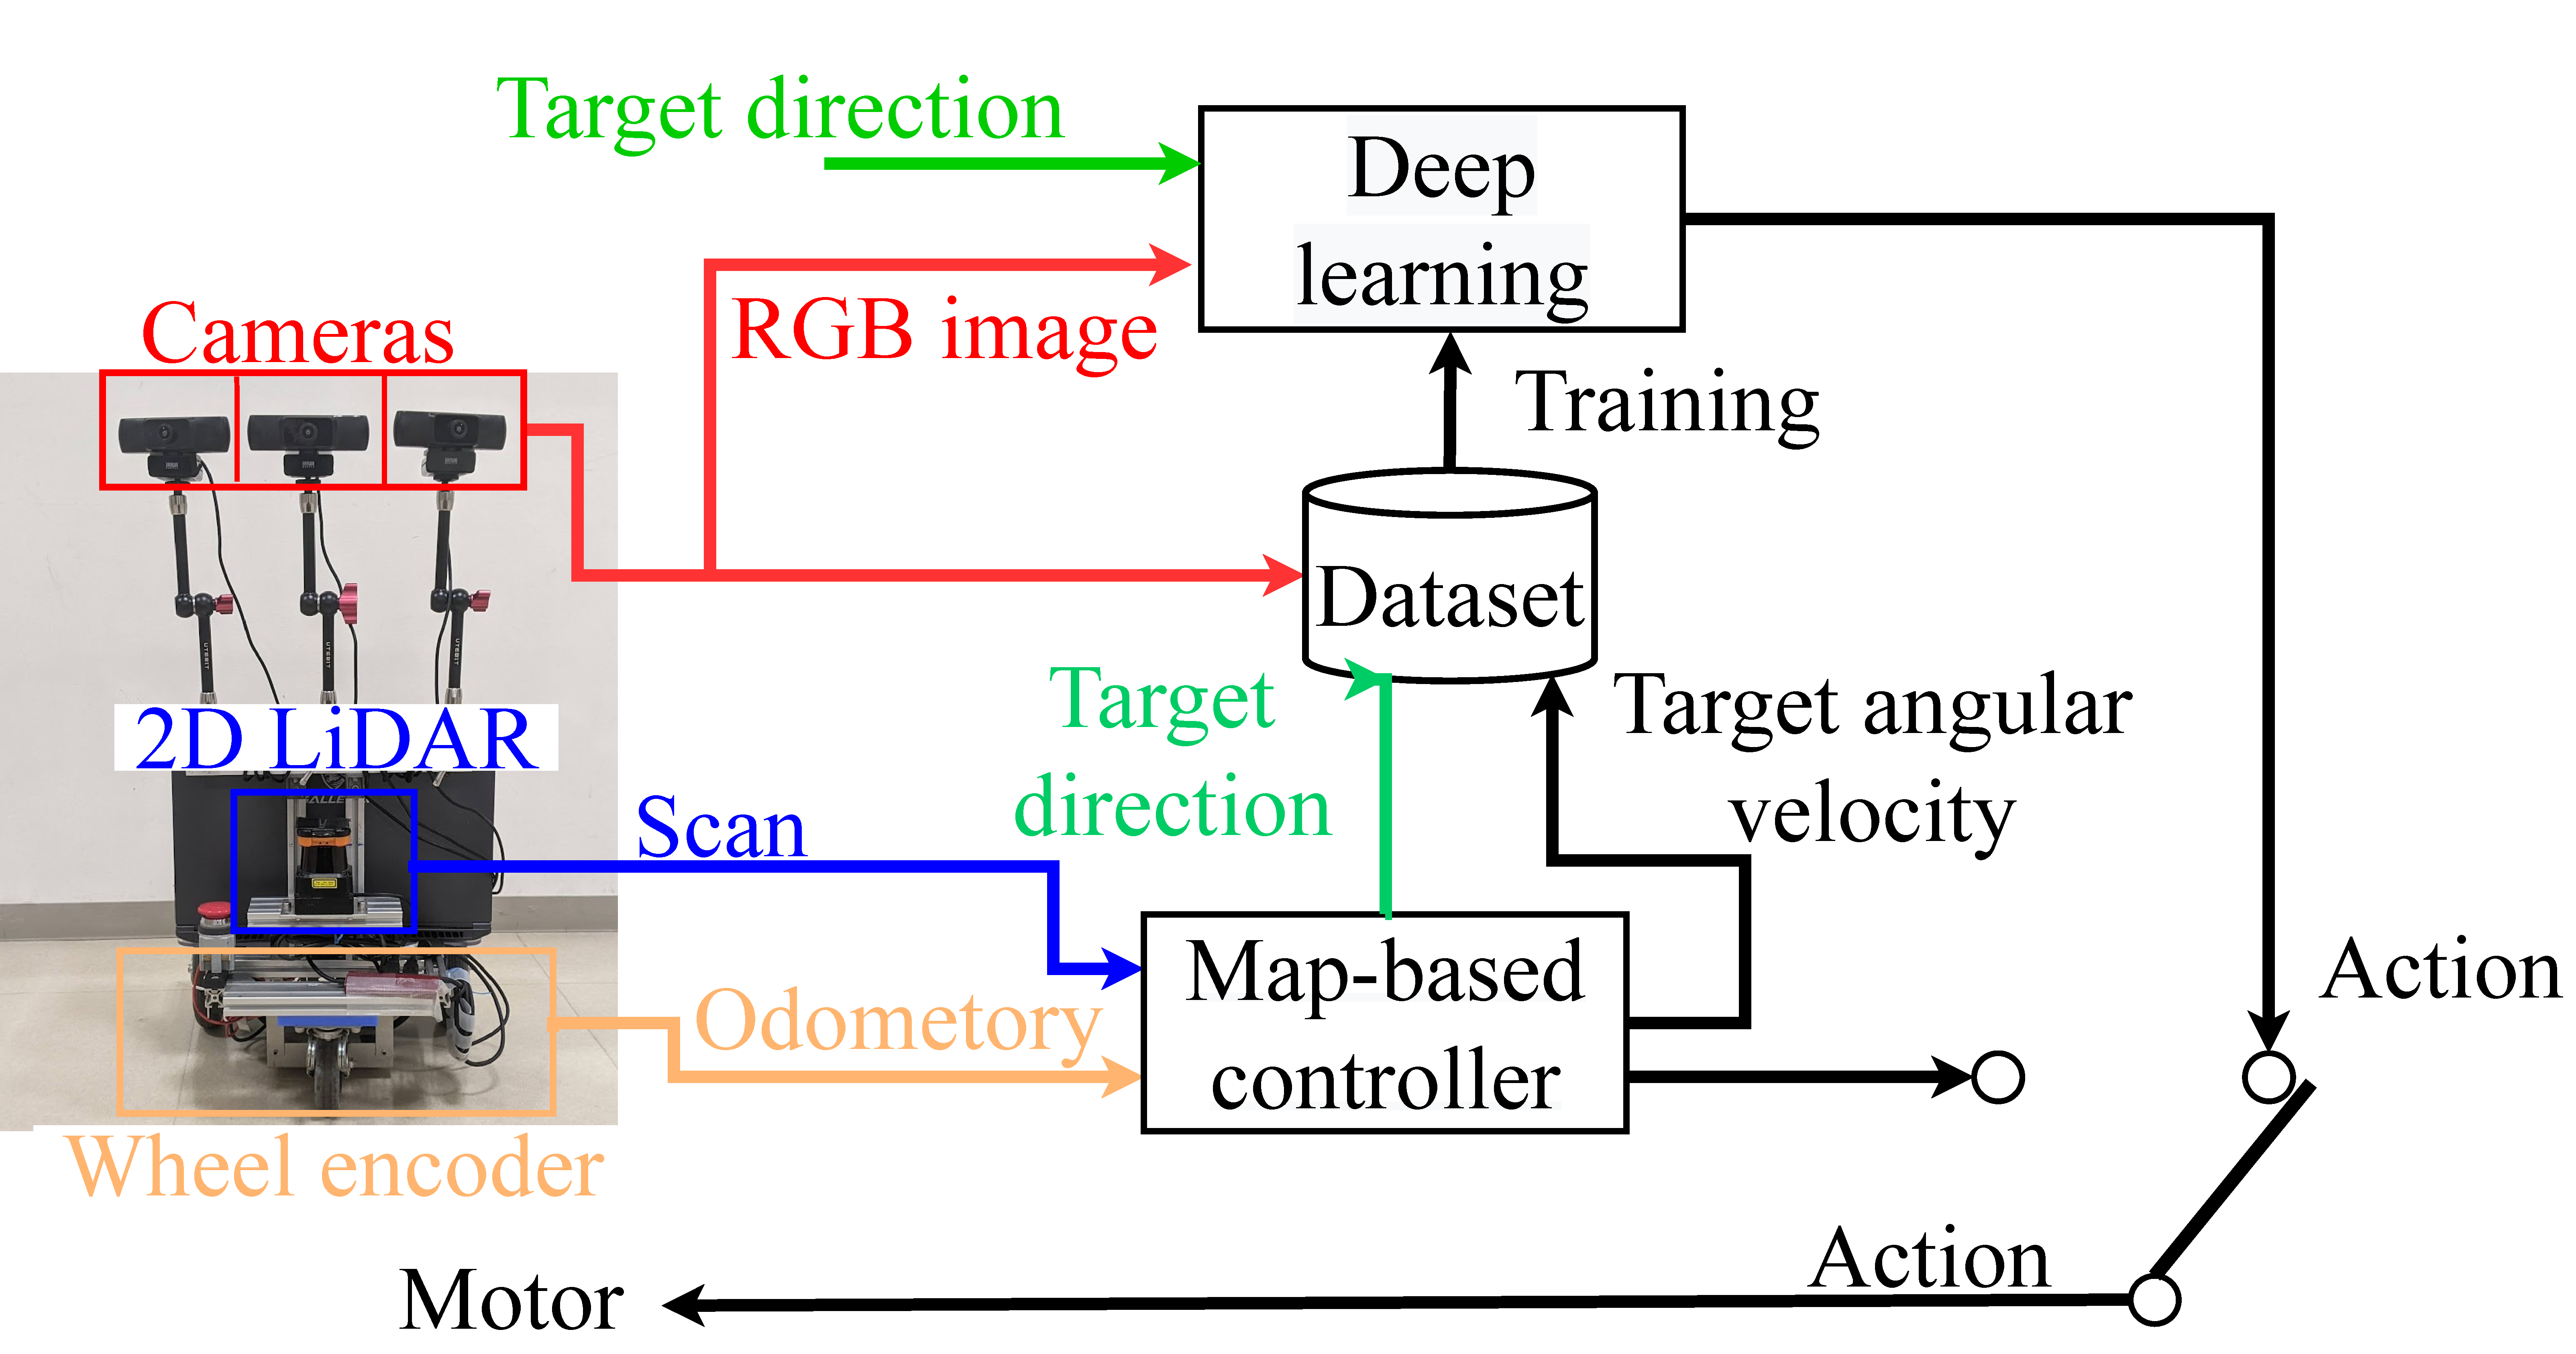
\includegraphics[width=130mm]{images/pdf/system_learning.pdf}
     \caption{Path-following module system}\label{fig:learning_sys}
\end{figure}

学習時のデータセットの収集には,
岡田ら\cite{okada2021}が提案した
\begin{quote}
    \begin{itemize}
     \item 学習器の出力を監視して,経路追従できない場所のデータのみ選択してデータセ
     ットに追加する手法
    \end{itemize}
   \end{quote}
及び藤原ら\cite{fujiwara2023}が提案した
\begin{quote}
    \begin{itemize}
     \item データセットに加えるデータの不均衡を改善する手法
     \item 学習時に積極的に蛇行する手法
    \end{itemize}
   \end{quote}

データセットに加えるデータの不均衡を改善する手法について述べる.
データ前処理手法であるオーバーサンプリングを用いて,データの偏りを改善する.
具体的には,直進,左折,右折のデータの中で,左折と右折を7倍に複製する.
次に,学習時に積極的に蛇行する手法について述べる.
この手法では\ref{fig:dakou}に示すように,学習時のロボットの制御に用いる目標角速度を1.5倍にする.これにより,大きく蛇行して,目標経路から離れた状態を
多く収集する.
\begin{figure}[htbp]
    \centering
     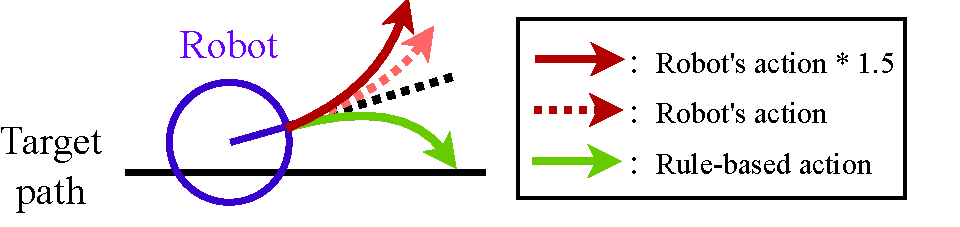
\includegraphics[width=130mm]{images/pdf/dakou.pdf}
     \caption{Aggressive meandering Quote from \cite{fujiwara2023}}\label{fig:dakou}
\end{figure}
\newpage
経路追従モジュールで用いるネットワークの構造を\ref{fig:imi_net}に示す.
ネットワークはRGB画像と,目標方向を入力,ヨー方向の角速度を出力として
end-to-endで学習する.
ネットワークは,画像を処理するCNNアーキテクチャ,CNNの出力と目標方向を入力とする全結合層で構成されている.
\begin{figure}[htbp]
    \centering
     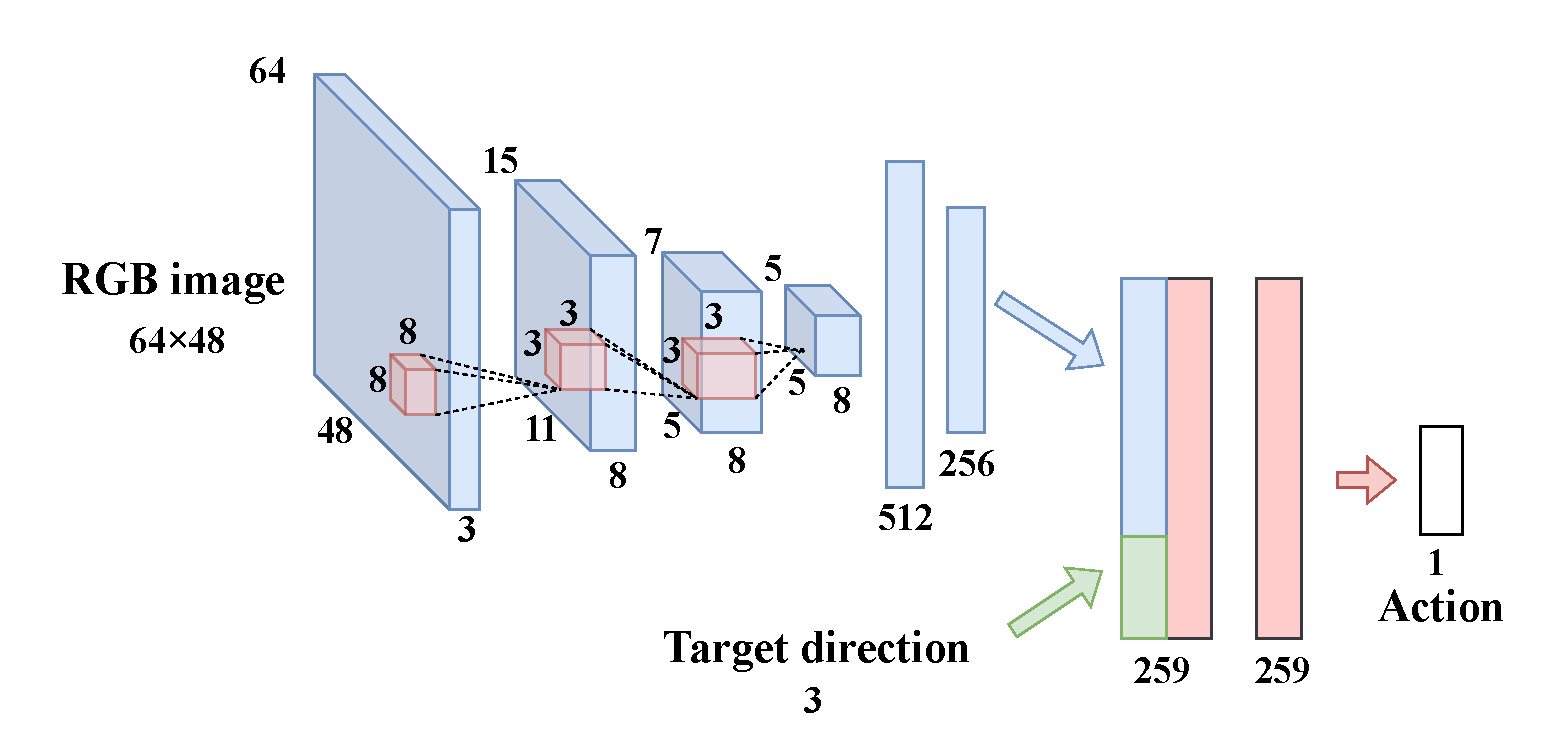
\includegraphics[width=130mm]{images/pdf/imi_net.pdf}
     \caption{Aggressive meandering}
     \label{fig:imi_net}
\end{figure}

目標方向は\ref{tab:target}に示す
直進,左折,右折の3つをワンホットベクトルとして入力する.
この中で,停止はネットワークへは入力せず,
この目標方向が停止の場合には,前述の通り並進速度,角速度ともに0.0m/sとする.
\begin{table}[htbp]
    \centering
    \caption{Target direction and data for path-following module}\label{tab:target}
    \begin{tabular}{|c|c|}
    \hline
    Target direction & Data        \\
    \hline
    Go straight   & {[}1,0,0{]} \\
    Turn left   & {[}0,1,0{]} \\
    Turn right   & {[}0,0,1{]} \\
    Stop   & {[}0,0,0{]}\\
    \hline
    \end{tabular}
    \end{table}